\subsection{Klient webowy}
\label{subsub:impl-webclient}

Klient webowy został zaimplementowany w obu aplikacjach jako statyczna strona internetowa, której kod JavaScript przechowany jest w Web Storage (podsekcja \ref{subsub:webstorage}) za pomocą basket.js (podsekcja \ref{subsub:tools-basketjs}). Komunikacja z serwerem została zrazlizowana przy pomocy biblioteki Socket.io (podsekcja \ref{subsub:socketio}), odbywa się ona za pomocą protokołu Web Sockets (podsekcja \ref{subsub:websockets}) lub w przypadku braku wsparcia z jedną ze wspieranych metod przez bibliotekę Socket.io z modelu Comet (podsekcja \ref{sub:communication-methods}). W aplikacjach wykrywane są dotknięcia ekranu urządzenia mobilnego (sekcja \ref{sub:touch-detection}) przy użyciu biblioteki jQuery Mobile (podsekcja \ref{subsub:tool-jquery-mobile}).

\subsubsection{Reprezentacja kursora na płaszczyźnie}
\label{subsub:cursor-representation}

Kursor jest reprezentowany za pomocą punktu \(C(x_{c}, y_{c})\) o nieujemnych, całkowitych współrzędnych \emph{cursor coordinate} oznaczających jego pozycję od punktu \(P(0, 0)\) umieszczonego w lewym, górnym rogu ekranu, a wektor jest skierowany ku punktowi w prawym, dolnym rogu ekranu.

\begin{figure}[h!]
  \caption{Sposób wyznaczania pozycji kursora myszy.}
  \centering
    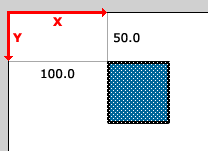
\includegraphics{wyznaczanie-pozycji-kursora}
\end{figure}

Uwzględniając różne proporcje \(p = \frac{szerokosc}{wysokosc}\) ekranu na którym pojawia się zdalnie sterowany kursor oraz proporcje powierzchni ekranu urządzenia mobilnego, w implementacji pilota użyta została reprezentacja procentowa punktu na ekranie.

Pozycja kursora reprezentowana jest przez punkt \(P(x, y)\) na dwuwymiarowej płaszczyźnie w zakresie \( x\in \langle0, 1\rangle \), gdzie \(x = \frac{x_{c}}{w_{x}}\), \(y = \frac{x_{c}}{w_{y}}\), a \(w_{x}\) oraz \(w_{y}\) oznaczają kolejno szerokość i wysokość ekranu.

Wyznaczanie pozycji uwzględnia również zmianę orientacji (poziomej lub pionowe), szerokości i wysokości rzutni okna przeglądarki wyświetlanej na urządzeniu mobilnym.

\lstset{language=JavaScript}
\begin{lstlisting}
this.run = function() {
	
	var this = that
	this.windowX = 0
	this.windowY = 0
	
	$(document).on('vmousemove', function(e) {
		e.preventDefault(); // prevent scroll
		
		var x = e.pageX / that.windowX
		var y = e.pageY / that.windowY
		
		console.log(x, y) // wypisz punkty
	})
	
	var indicateWindowSize = function() {
		that.windowX = $(window).width()
		that.windowY = $(window).height()
	}
	
	// register window size changes listeners
	$(window).on('resize orientationchange', function() {
		indicateWindowSize()
	})
	indicateWindowSize()
}
\end{lstlisting}

\subsubsection{Pilot do sterowania zdalnym monitorem}

Logika aplikacji pilota jest trywialna. Przechwytuje punty zestyku użytkownika z urządzeniem mobilnym, przekształca reprezentację współrzędnych (podsekcja \ref{subsub:cursor-representation}) i wysyła do je do serwera w postaci współrzędnych x, y za pomocą metody \lstinline{emit()} biblioteki socket.io (podsekcja \ref{subsub:socketio}) wiadomością o temacie \emph{mouseMoveToPercent}:

\lstset{language=JavaScript}
\begin{lstlisting}
this.run = function() {
	// init socket connection
	that.socket = socketConnect(that.socket, that.serverAddress);
	
	that.socket.emit('connectToRemote', {
		host: that.serverRemoteHost,
		port: that.serverRemotePort
	})
	
	// register listeners
	$(window).on('resize orientationchange', function() {
		indicateWindowSize()
	})
	indicateWindowSize()
	
	$(document).on('vmousemove', function(e) {
		e.preventDefault(); // prevent scroll
		
		var x = e.pageX / that.windowX
		var y = e.pageY / that.windowY
		
		if(that.x == null || that.y == null || Math.abs(that.x - x) > that.minDelta || Math.abs(that.y - y) > that.minDelta) {
			that.x = x
			that.y = y
			
			var data = {
				x: x,
				y: y
			}
			
			that.socket.emit('mouseMoveToPercent', data)
		}
	})
}
\end{lstlisting}

Aplikacja posiada również zapisy konfiguracji (nazwa hosta oraz port) połączenia do serwera programu generującego zdarzenia urządzeń wejścia (podsekcja \ref{sub:impl-displayclient-events-dispatcher}), do którego ma być przekazywana pozycja, którą wysyła wiadomością o temacie \emph{connectToRemote}. Przykładowa konfiguracja\footnote{Pełen opis instalacji w podsekcji \ref{subsub:setup-server-nodejs}}:

\lstset{language=HTML}
\begin{lstlisting}
<body data-server="192.168.1.127:8080" data-server-remote-host="192.168.1.127" data-server-remote-port="8081">
</body>
\end{lstlisting}

Interfejs wyjściowy aplikacji:

\begin{description}
	\item[mouseMoveToPercent] \hfill \\
	Komunikat wysyłany do serwera, informujący o pozycji kursora.
	\begin{enumerate}
		\item x (float)
		\item y (float)
	\end{enumerate}
\end{description}

\begin{description}
	\item[connectToRemote] \hfill \\
	Komunikat wysyłany do serwera, informujący o połączeniu do serwera programu generującego zdarzenia urządzeń wejścia.
	\begin{enumerate}
		\item host (string)
		\item port (float)
	\end{enumerate}
\end{description}

Interfejs wejściowy aplikacji:

Brak.

\subsubsection{Pilot gry PONG wyświetlanej na zdalnym monitorze}

Pilot do sterowania grą PONG wyświetlaną na zdalnym monitorze umożliwia zgłoszenie chęci uczestnictwa w grze oraz sterowanie paletką. Na ekranie startowym użytkownik widzi przycisk, dzięki któremu może zgłosić chęć uczestnictwa w grze, następnie pilot wyświetla komunikaty, aż wreszcie umożliwia sterowanie paletką. Aplikacja jest napisana w jQuery oraz ostylowana arkuszem napisanym w CSS 3.

Interfejs wyjściowy aplikacji:

\begin{description}
	\item[paddleMove] \hfill \\
	Komunikat informujący serwer o zmianie położenia punktu zestyku użytkownika z ekranem:
	\begin{enumerate}
		\item positionX (float)
		\item positionY (float)
	\end{enumerate}
\end{description}

Interfejs wejściowy aplikacji (komunikaty wysyłane przez serwer do klienta):

\begin{description}
	\item[signalCurrentServerState] \hfill \\
	Komunikat informujący o stanie gry oraz kolejki. Odbierany jest za każdym razem, gdy zmienia się stan gry: ilość użytkowników oczekujących na grę, włączenie gry. Na podstawie otrzymanych danych wyświetla się komunikat, który w kolejce jest użytkownik.
	\begin{enumerate}
		\item count (int) ilość użytkowników oczekujących w kolejce do gry
		\item isGame (boolean) informacja, czy jest rozgrywana gra, czy nie
	\end{enumerate}
\end{description}

\begin{description}
	\item[signalWaitingForPartner] \hfill \\
	Komunikat oznaczający, że klient został przyjęty do kolejki oczekujących graczy i oczekuje na partnera do gry.
\end{description}

\begin{description}
	\item[welcome] \hfill \\
	Komunikat oznaczający, że klient rozpoczyna grę.
\end{description}

\begin{description}
	\item[gameOver] \hfill \\
	Komunikat wysyłany przez serwer informujący o zakończeniu gry. Na podstawie otrzymanych danych wyświetla się informacja, czy klient przegrał, czy wygrał.
	\begin{enumerate}
		\item score (int) wynik klienta
		\item scoreEnermy (int) wynik przeciwnika
	\end{enumerate}
\end{description}
